\PassOptionsToPackage{unicode=true}{hyperref} % options for packages loaded elsewhere
\PassOptionsToPackage{hyphens}{url}
%
\documentclass[]{article}
\usepackage{lmodern}
\usepackage{amssymb,amsmath}
\usepackage{ifxetex,ifluatex}
\usepackage{fixltx2e} % provides \textsubscript
\ifnum 0\ifxetex 1\fi\ifluatex 1\fi=0 % if pdftex
  \usepackage[T1]{fontenc}
  \usepackage[utf8]{inputenc}
  \usepackage{textcomp} % provides euro and other symbols
\else % if luatex or xelatex
  \usepackage{unicode-math}
  \defaultfontfeatures{Ligatures=TeX,Scale=MatchLowercase}
\fi
% use upquote if available, for straight quotes in verbatim environments
\IfFileExists{upquote.sty}{\usepackage{upquote}}{}
% use microtype if available
\IfFileExists{microtype.sty}{%
\usepackage[]{microtype}
\UseMicrotypeSet[protrusion]{basicmath} % disable protrusion for tt fonts
}{}
\IfFileExists{parskip.sty}{%
\usepackage{parskip}
}{% else
\setlength{\parindent}{0pt}
\setlength{\parskip}{6pt plus 2pt minus 1pt}
}
\usepackage{hyperref}
\hypersetup{
            pdfauthor={Zhenghong Lieu},
            pdfborder={0 0 0},
            breaklinks=true}
\urlstyle{same}  % don't use monospace font for urls
\usepackage{graphicx,grffile}
\makeatletter
\def\maxwidth{\ifdim\Gin@nat@width>\linewidth\linewidth\else\Gin@nat@width\fi}
\def\maxheight{\ifdim\Gin@nat@height>\textheight\textheight\else\Gin@nat@height\fi}
\makeatother
% Scale images if necessary, so that they will not overflow the page
% margins by default, and it is still possible to overwrite the defaults
% using explicit options in \includegraphics[width, height, ...]{}
\setkeys{Gin}{width=\maxwidth,height=\maxheight,keepaspectratio}
\setlength{\emergencystretch}{3em}  % prevent overfull lines
\providecommand{\tightlist}{%
  \setlength{\itemsep}{0pt}\setlength{\parskip}{0pt}}
\setcounter{secnumdepth}{0}
% Redefines (sub)paragraphs to behave more like sections
\ifx\paragraph\undefined\else
\let\oldparagraph\paragraph
\renewcommand{\paragraph}[1]{\oldparagraph{#1}\mbox{}}
\fi
\ifx\subparagraph\undefined\else
\let\oldsubparagraph\subparagraph
\renewcommand{\subparagraph}[1]{\oldsubparagraph{#1}\mbox{}}
\fi

% set default figure placement to htbp
\makeatletter
\def\fps@figure{htbp}
\makeatother

\usepackage[]{natbib}
\bibliographystyle{plainnat}

\author{Zhenghong Lieu}
\date{}

\begin{document}

\begin{quote}
spatial diversity remained a statistically significant predictor of
roll-off rate. With these variables held constant at their means, a
House district's shift from the tenth to the ninetieth percentile in
spatial diversity was associated with an increase in roll-off rate of
about six percentage points
\end{quote}

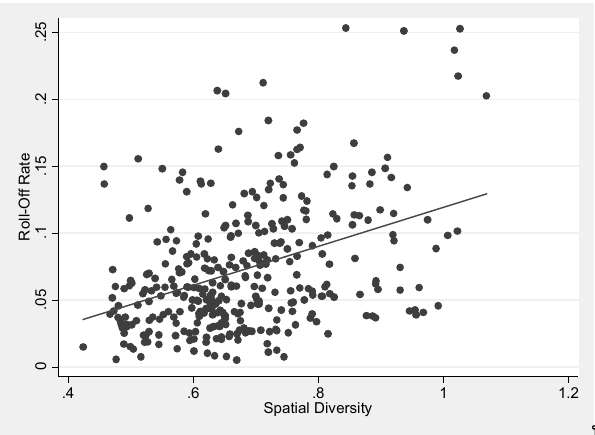
\includegraphics{img/sd_rolloff.png}

\cite{steph2012}

\hypertarget{overview-of-research-strategy}{%
\subsection{Overview of research
strategy}\label{overview-of-research-strategy}}

Two key research questions:

\begin{enumerate}
\def\labelenumi{\arabic{enumi}.}
\tightlist
\item
  Do more compact districts have better, equal, or worse spatial
  diversity scores?
\item
  Is there an inherent trade-off between compactness and homogeneity?
\item
  Does spatial diversity give us a normative basis to select one
  compactness metric over another?
\end{enumerate}

The research procedure:

\begin{enumerate}
\def\labelenumi{\arabic{enumi}.}
\item
  Generate a large and representative subset of plausible districting
  plans
\item
\end{enumerate}

\hypertarget{overview-of-compactness-measures}{%
\subsubsection{Overview of compactness
measures}\label{overview-of-compactness-measures}}

To empirically evaluate a trade-off between compactness and homogeneity,
we must first define the metrics by which we evaluate a proposed
districting plan over each of these dimensions. Here, I introduce many
different compactness measures. I give a brief overview of the different
types of measures, explain the pros and cons of each, present a
compactness measure that I develop, and support my decision to use an
ensemble of measures to increase robustness.

\hypertarget{geometric-compactness-metrics}{%
\paragraph{Geometric compactness
metrics}\label{geometric-compactness-metrics}}

Shape-based versus dispersion-based

The most

\hypertarget{polsby-popper}{%
\paragraph{Polsby-Popper}\label{polsby-popper}}

The Polsby-Popper measure, introduced by Polsby and Popper in 1991, is a
ratio of the area of the district to the area of a circle whose
circumference is equal to the perimeter of the district.

\[4\pi \times \frac{A}{P^2}\]

\begin{figure}
\centering
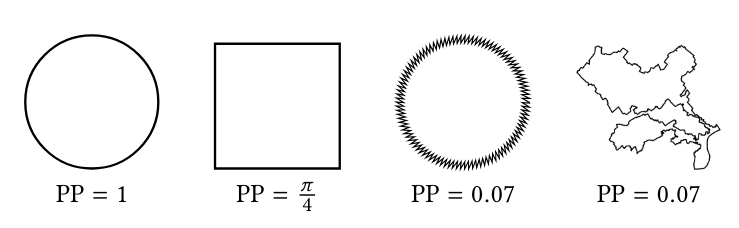
\includegraphics{img/pp_example.png}
\caption{Polsby-Popper scores of four example regions: a perfect circle,
a square, a circle with a ragged boundary, an an example district from a
Pennsylvania plan. Taken from \cite{s2020}.}
\end{figure}

\hypertarget{reock}{%
\paragraph{Reock}\label{reock}}

The Reock score is a measure of the ratio of the district to the area of
the minimum bounding circle that encloses the district's geometry.

\[\frac{Area}{AreaOfMinimumBoundingCircle}\]

\hypertarget{convex-hull}{%
\paragraph{Convex Hull}\label{convex-hull}}

The Convex Hull metric is a ratio of the area of the district to the
area of the minimum convex polygon that can enclose the district's
geometry.

\[\frac{Area}{AreaOfMinimumConvexPolygon}\]

\hypertarget{choosing-a-compactness-metric}{%
\paragraph{Choosing a compactness
metric}\label{choosing-a-compactness-metric}}

Which compactness measure should we choose? All three compactness
measures are well-cited in the literature and enjoy widespread use. They
have been cited in U.S. Supreme Court cases, \emph{amici} briefs, and
redistricting commissions \citep{moncrief2011}. Despite their widespread
acceptance, however, the problems with compactness measures are many,
and well-covered in the literature. No compactness measure is perfect:
as an example, the most popular compactness measure in the
literature---Polsby-Popper---is sensitive to small perturbations in data
resolution (the coastline problem). \footnote{The Polsby-Popper metric
  measures the ratio of the area of the district to the area of a circle
  whose circumference is equal to the perimeter of the district. But
  depending on the resolution of the map, the perimeter can be
  effectively infinite. \citeauthor{bswp} find that the choice of
  resolution has ``a substantial impact on compactness scores, with the
  Polsby-Popper score especially affected.''} It is therefore important
to use an \emph{ensemble} of compactness measures to make sure that
one's data and conclusions are robust.

But even this is not enough. Because most compactness measures are
purely geometric, they are all vulnerable to a specific family of
geographic perturbations. Indeed, \cite{bswp} show that minimally
tweaking the geometric features of states is enough for the four most
popular compactness measures (Polsby-Popper, Convex Hull, Reock,
Schwartzberg) to give very different conclusions on nominally identical
data.

Thus, it is important to include a non-geometric compactness measure in
the ensemble to guard against the possibility that the results are
driven by a specific quirk in geography. Many such measures have been
proposed. For instance, \cite{dc2016} bring in a discipline of
mathematics---graph theory---to formulate a new metric of compactness.

However, one particular class of metrics I term \emph{point-wise
distance metrics} stands out for its ease of understanding (critical if
it is to be persuasive to Supreme Court judges), theoretical
attractiveness, and academic consensus. This class of compactness
metrics tries to measure the distance between two voters in a district,
and assigns higher scores the lower that distance is.

This class of metrics enjoy strong theoretical grounding. Paramount to
the idea of single-member districts is that there is some value in
voters who live in the same area being put into the same district.
\cite{er2019}:

\begin{quote}
``Voters in the same area are likely to share political interests;
voters in the same area are better able to communicate and coordinate
with one another; politicians can better maintain connections with
voters in the same area; voters in the same area are especially likely
to belong to the same social communities --- all suggest the importance
of voters being located in districts with their geographic peers.''
\end{quote}

In contrast, districts that carve voters out of their natural
communities and pool them with unrelated, distant voters are bad ones.
Therefore, we should be sensitive not just to geometric shape, but
rather whether or not voters live close to one another. This class of
metrics is more readily understandable to laymen and possesses a
normative bent that more abstract mathematical compactness measures
lack. It has therefore been an active area of development in the
literature. \cite{cm2010} present a measure of ``bizarreness'', which is
the ``expected relative difficulty in traveling between two points
within the district''. And \cite{fh2011} measures ``the distance between
voters within the same district relative to the minimum distance
achievable''.

\citeauthor{fh2011}'s approach is however an NP-hard problem

I make two key improvements to existing metrics. First, I use driving
durations rather than Euclidean (as-the-crow-flies) distances between
voters. This keeps the metric robust to quirks in political geography
like mountains and lakes, and better represents the notion of natural
communities. This idea is not new and has been discussed in the
literature. In fact, while \cite{fh2011} used Euclidean distance in his
metric, he points out its shortcomings:

\begin{quote}
Suppose there is a city on a hill. On the West side is {[}a{]} mild,
long incline toward the rest of the city, which is in a plane. On the
East side is a steep cliff, either impassable or with just a narrow,
winding road that very few people use. While the next residential center
to the East is much closer to the hilltop on a horizontal plane, it is
much further on all sorts of distances that we think might matter:
transportation time, intensity of social interactions, sets of shared
local public goods and common interests, etc. Thus, for all practical
purposes, one probably wants to include the hilltop in a Western
district rather than an Eastern one. More general notions of distance
can handle this.
\end{quote}

In this case, driving durations would better reflect this quirk in
political geography. The ``impassable'' region on the East would have a
short Euclidean distance, and any districting plan that put the hilltop
with the Eastern district would be unfairly penalised by these
point-wise distance metrics. On the other hand, the impassable region
would have a long driving duration, accurately reflecting the political
geography. In fact, \citeauthor{fh2011} specifically suggest using
driving durations to improve their metric: ``one can extend much of
{[}our analysis{]} by using driving distance or what legal scholars
refer to as `communities of interest'\,''.

The use of driving durations seems strictly superior in many cases
involving human-scale distances. Working with Nicholas Eubank and
Jonathan Rodden, I update their gerrymandering-detection metric to use
driving durations instead \citep{er2019}. We find a consistently
different picture of the social context of American suburban voters,
raising the possibility of false positives under the Euclidean distance
measure \citep*{elrwp}.

Why then have

Similar concerns were echoed by Brian Olson, the creator of
BDistricting, who also chose to use Euclidean distances rather than
driving durations because: ``It might be the right kind of thing to
measure, but it would take too long\ldots{} the large amount of map data
and extra computer time to calculate all those travel times would slow
the process down horribly. It would then require a room filling
supercomputer to get an answer in a reasonable amount of time''.

Therefore, while many have recognised the theoretical advantages of
using travel times over Euclidean distances / geographic compactness, no
one has of yet come up with a computationally feasible way to use it. By
adopting techniques like downsampling, memoisation, and the use of data
structures from computer science, I can make the calculation of travel
times computationally feasible, and (hopefully) competitive with
existing compactness algorithms like Convex Hull or Polsby-Popper.

that builds upon all these approaches. In \cite{elrwp}, we

Secondly,

Further details on the metric can be found in Appendix A.

As a result,

As the Schwartzberg and Polsby-Popper measure are mathematically
equivalent, I include only Polsby-Popper in the ensemble.

I therefore have what I believe to be the most robust ensemble of
compactness measures in the literature

\hypertarget{human-compactness}{%
\paragraph{Human compactness}\label{human-compactness}}

\hypertarget{overview-of-automated-districting-algorithms}{%
\subsubsection{Overview of automated districting
algorithms}\label{overview-of-automated-districting-algorithms}}

In order to find out whether compactness measures track spatial
diversity, we have to generate many counterfactual plausible plans that
span the entirety of possible districting plans and measure the
correlation between compactness and spatial diversity. This requires
using a computer to draw a large number of plans according to some
minimal criteria.

The idea of drawing a large number of districting plans with a computer
has a long and storied history, starting in the 60s and 70s. The
approach has almost always been used to identify gerrymandering; for
instance \cite{ccd2000} build an algorithm to ``quantitatively
{[}assess{]} whether the {[}1990 South Carolina{]} plan is a racial
gerrymander''. More recently, \cite{cr2013} ``generat{[}e{]} a large
number of hypothetical alternative districting plans that are blind as
to party and race, relying only on criteria of geographic contiguity and
compactness.'' They do this using a Markov Chain simulation algorithm, a
procedure that makes iterative changes for a large number of steps until
a unique districting plan emerges. At each step of
\citeauthor{ccd2000}'s algorithm, they randomly select a Census Block
Group to serve as a ``seed'' of the district, then randomly add its
neighbouring block groups to it until a district with the desired
population is formed. Similarly, \citeauthor{cr2013} begin by
initialising all precincts as an individual, separate district, then
randomly agglomerating neighbouring precincts until the desired number
of districts is reached.

While this ``standard simulation algorithm'' enjoys a certain degree of
success, it has one crippling weakness. The way in which this class of
algorithms operates necessarily explores only a tiny subset of all
possible districting plans. Subsequent work pointed out this flaw:
\citeauthor{mm2018} wrote that automated processes ``may take a biased
sample of all possible legislative maps\ldots{} and fail to efficiently
produce a meaningful distribution of all alternative maps''. And
\citeauthor{fifieldwp} contend that ``{[}standard Monte Carlo
algorithms{]} are unlikely to yield a representative sample of
redistricting plans for a target population.'' \footnote{See
  \cite{fifieldwp}, pg. 16, for a technical explanation of why these
  algorithms don't produce uniform redistricting plans: ``For example
  \ldots{}, the creation of earlier districts may make it impossible to
  yield contiguous districts. These algorithms rely on rejection
  sampling to incorporate constraints, which is an inefficient strategy.
  More importantly, the algorithms come with no theoretical result and
  are not even designed to uniformly sample redistricting plans.''} This
poses a huge issue for the validity of any statistical analysis, because
any correlation that we discover on a biased subset of plans may be
spurious when measured over the actual distribution of plans. \footnote{Generating
  a biased sample is not necessarily a problem if all you want to do is
  \emph{optimise}, e.g.~draw the most compact plan possible. Recent work
  builds upon this standard algorithm, using Voronoi diagrams or
  iterative flood fill procedures rather than random chance, to assign
  the precincts to be agglomerated. See \cite{lf2019} for a technical
  overview.}

Thankfully, scholars have developed an improvement over the standard
algorithm with stronger theoretical guarantees. This second class of
algorithms reframe the districting problem as a \emph{graph partition}
problem (borrowing insights from graph theory and computer science), and
use a \emph{Markov Chain Monte Carlo} (MCMC) approach to sample possible
districting plans. This approach is best laid out in \cite{fifieldwp}.
Broadly speaking, the approach initialises a specific graph partition as
a step in the Markov Chain, then \emph{flips} a random node of the graph
to get another valid partition. This process is repeated until the
Markov Chain approaches its steady state distribution: when this
happens, the Markov chain is called ``well-mixed''.

This class of algorithms inherit desirable well-known theoretical
guarantees of the Markov Chain.\footnote{See \cite{ddj2019recom} for a
  technical overview} They are therefore much less likely (both
theoretically and empirically) to generate a biased subset of plans.
Conducting a small-scale validation study on a 25-precinct set,
\citeauthor{fifieldwp} compare the distribution of plans generated by
their algorithm to those generated by the standard redistricting
algorithm. They prove that their algorithm produces plans that hew much
more closely to the \emph{actual} distribution of all possible
districting plans.

Due to the many advantages of the MCMC approach, I use it in all my
analyses. I use an superior proposal distribution called Recombination
(Recom) by \citeauthor{ddj2019recom}, which uses a spanning tree method
to bipartition pairs of adjacent districts at each step
\citep{ddj2019comp}. This proposal distribution improves upon the
\texttt{Flip} proposal in \citeauthor{fifieldwp} in two significant
ways: it generates plans in much fewer steps \footnote{the ``mixing
  time'' of the Markov Chain---that is, the number of steps it takes for
  the Markov Chain to be ``close enough'' to the stationary
  distribution---is order of magnitudes smaller in \texttt{Recom}
  compared to \texttt{Flip}.}, and it generates plans that are much more
realistic. The \texttt{Flip} proposal tends to generate very uncompact,
snakelike districts, as can be seen in the figure.

\begin{figure}
\centering
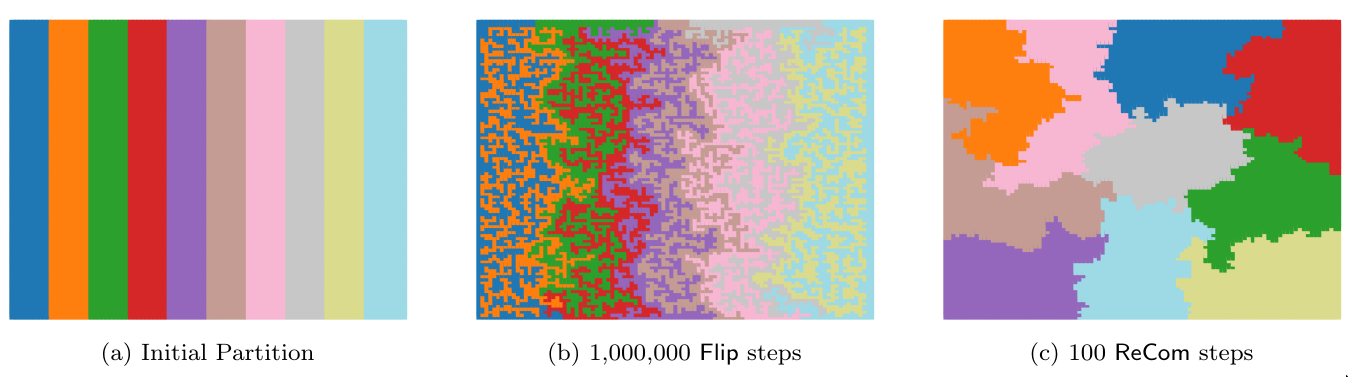
\includegraphics{img/recom_vs_flip.png}
\caption{The \texttt{Recom} proposal generates more realistic plans in
much fewer steps. Taken from \cite{ddj2019recom}.}
\end{figure}

\hypertarget{data-generation}{%
\subsection{Data generation}\label{data-generation}}

\begin{enumerate}
\def\labelenumi{\arabic{enumi}.}
\tightlist
\item
  Generate 100,000 districting plans
\end{enumerate}

I download Census Tract level. These can be downloaded from the
\href{census.gov}{United States Census Bureau} website.

I use the open-source software library GerryChain to generate the
ensembles. Replication code and data are included in the Supplementary
Information. I obtain the ReCom Markov chain procedure from one of the
co-authors of the \cite{ddj2019recom} paper, and generate 10,000
districting plans for 10 states (Connecticut, Georgia, Idaho, Louisiana,
Maine, Maryland, New Hampshire, Rhode Island, Utah, and Wisconsin) for a
total of 100,000 plans.

\begin{enumerate}
\def\labelenumi{\arabic{enumi}.}
\setcounter{enumi}{1}
\tightlist
\item
  Calculate spatial diversity and compactness scores for each of the
  100,000 districting plans
\end{enumerate}

I obtain data on spatial diversity from Professor Nicholas
Stephanopoulos

In order to keep the calculation of human compactness to a reasonable
time, I first precalculate a \emph{duration matrix} for every state:
this gives the point-to-point driving durations from each voter to every
other voter in the state. In order to

I obtain voter data from \citeauthor{er2019},

In order to do this, I have to

\begin{enumerate}
\def\labelenumi{\arabic{enumi}.}
\setcounter{enumi}{2}
\tightlist
\item
  Analyse
\end{enumerate}

\hypertarget{discussion-and-future-work}{%
\subsection{Discussion and future
work}\label{discussion-and-future-work}}

\hypertarget{appendix-a-calculation-of-human-compactness}{%
\subsection{Appendix A: Calculation of human
compactness}\label{appendix-a-calculation-of-human-compactness}}

\hypertarget{very-similar-paper}{%
\subsection{Very similar paper}\label{very-similar-paper}}

We posit that this is due to thepolitical geographies of the two states,
and examining this effect isan important thread for understanding what
kinds of reforms mightor might not be effective in various
jurisdictions. Future work coulduse more sophisticated mathematical and
statistical techniques todescribe a relationship between political
geography and the trade-offs we consider here. Our analysis suggests
that a one-size-fits-allapproach to drawing `fair' districts is
inappropriate and that indi-vidual states and localities should
carefully consider the relevanttrade-offs when redistricting or
implementing redistricting reforminitiatives. One factor ignored in this
analysis, which is critical to theprocess of drawing districts,
isrespecting communities-of-interest.Even defining and locating
geographically such communities is avery difficult problem, let alone
the determination of whether ornot to preserve that group in a single
district. We therefore pro-pose our analysis as a framework for
discussion about trade-offs inredistricting rather than as a policy
recommendation.In this work, we have demonstrated with a simple model
thatdemanding districts be drawn to be as compact as possible
anddemanding that they satisfy a notion of partisan symmetry
areincompatible, but to different degrees depending on the
particularfeatures of the geographic region in question. Since existing
propos-als and methodologies for automated and algorithmic
redistrictinginvolve finding an approximate solution to an optimization
problem,it is important to understand how changing the objective
functionof these procedures can affect the outcome. As more
jurisdictionsconsider redistricting reforms, they should be cautious
about abdi-cating the line drawing process to algorithms which encode
valuesdifferent from those of the voters who use the districts to elect
theirrepresentatives.

\bibliography{references.bib}

\end{document}
